\section{A Modern Approach to Seismic Data: Efficiency and Reproducibility}
\label{sec:asdf}
%\red{Wenjie}

Seismology is a science driven by observing, modeling, and
understanding data. In recent years, large volumes of high-quality seismic data
are becoming more and more easily accessible through the dramatic growth of
seismic networks. Together with the development of modern compute platforms,
both large-scale seismic simulations and data processing can be done
very efficiently. However, the  seismological community is not yet ready to
embrace the era of big data. Most seismic data formats and processing
tools were developed more than a decade ago and are becoming obsolete in many
aspects. In this chapter, we present our thoughts and efforts in bringing
modernity into the realm.

%\subsection{Introduction}

The very basic unit of seismic data is the seismogram, which is a time series of
ground motion recorded by a seismometer during an earthquake. Most seismometers on
land are able to record 3-component data: one vertical component, and two
horizontal components perpendicular to each other(usually east and north) while
seismometers in the ocean vary, some are equipped with a water pressure sensor and
others record 3-component displacement of the seabed (an Ocean Bottom
Seismometers). Seismometers are recording 7/24 and data are archived at data
centers. The data we are primarily interested in are 3-hour time windows after
an earthquake, during which time seismic waves propagate inside the
earth and gradually damp out.

\subsection{Legacy}

Most earthquake seismologists are familiar with Seismic Analysis Code (SAC, see
\cite{HelffrichWookeyBastow201311}), a general-purpose program designed for the
study of time series. It provides basic analysis capabilities, including general
arithmetic operations, Fourier transforms, filtering, signal stacking,
interpolation and etc., which fit the general requirements of researchers.

Alongside the software package, SAC also defines a data format, which has been
widely used by seismologists over the last few decades. In the SAC data format,
each waveform (time series) is stored as a separate data file, containing a
fixed length header section to store metadata, including time and location
information), followed by the data section (the actual time series). Thus, for
one earthquakes recorded by 2,000 seismometers, one would expect 6,000 independent
SAC files. The main reason SAC is popular within the seismological
community is its ease of use and its interactive command line tools. Even though
functionality is limited, SAC covers the most frequent needs of
seismologists. For example, visualizing seismograms is very easy in SAC and is
frequently used to check the effect of operations applied to data.
% What is more, considering the resource, both on data availability and
% computation power, are quite limited, even though the definition SAC data format
% is simple, it is sufficient for users at that time.

However, things are evolving quickly as more and more seismometers are
installed. For a single network, the number of seismometers can go easily beyond
$1,000$, leading to sizable datasets. Thus, SAC and its associated format is
no longer a good choice for the following reasons.
\begin{itemize}
    \item It has limited non-programmable functionalities.
      SAC tools have to be invoked by system calls (shell scripts) and the lack of APIs for programming
      languages, such as C and Fortran, makes it difficult to customize workflows.
    \item The SAC data format only stores one waveform per file.
      Given 5,000 earthquakes and 2,000 stations for each earthquake,
      $3*10^7$ SAC files have to be generated and stored. Reading or
      writing such a large number of files is highly inefficient,
    \item The header in the SAC data format is very limited, with only
      a fixed number of pre-defined slots to store metadata. However, a modern
       data format should be flexible enough for users to define metadata relevant to
       the problem they are solving. Imposing pre-defined offsets in bytes
       to access information is a recipe for disaster.
    \item Station information, which contains instrument response information,
    is stored in separate files. This approach increases the number of files to deal
    with and the possibility of making errors.
    Having the ability to store station information along with the waveform data
    greatly reduce the chances of mistakes.
\end{itemize}

\subsection{The Adaptable Seismic Data Format}

We looked for existing solutions lacking the drawbacks listed in the previous
paragraph.
Because introducing a new data format should ideally be avoided,
the seismological community has been postponing the
definition of more modern approaches.
We believe that the advantage of a new data format are significant
enough to quickly outweigh the initial difficulties of switching to a new
format. We identify five key issues that the new data format must resolve.
\begin{itemize}
  \item \textbf{Robustness and stability}: The data format should be stable enough
  to be used on large datasets while ensuring data integrity and the correctness of scientific results.
  \item \textbf{Efficiency}: The data format should be exploitable by efficient, parallel tools.
  \item \textbf{Data Organization}: Different types of data (waveform, source \& station information,
    derived data types) should be grouped at certain levels to perform a variety of tasks. The data
   should be self-describing so no extra effort is needed to understand the data.
  \item \textbf{Reproducibility}: A critical aspect of science is the ability to reproduce
    results. A modern data format should facilitate and encourage this.
  \item \textbf{Mining and Visualization of data}: Data could be queried and visualized anytime
    in an easy manner.
\end{itemize}

The Adaptable Seismic Data  Format (ASDF)~\cite{krischer2016adaptable} was introduced to
solve these issues.
Using HDF5 at its most basic level, it organizes its data in a hierarchical
structure inside a container ---in a simplified manner a container can be
pictured as a file system within a file.

HDF5 was chosen as the underlying data format for a variety of reasons.
First, HDF5 has been used in a wide variety of scientific projects and
has a rich and active ecosystem of libraries and tools. It has a number of
built-in data compression algorithms and data corruption tests in the form of
check summing.
Second, it also fulfills our hard requirement of being capable of parallel I/O
with MPI~\cite{MPI, Howison2010}.
Besides, there is no need to worry about the endianness of data, which
historically has been a big issue in seismology.

An ASDF file is roughly arranged in four sections, as follows.
\begin{enumerate}
    \item Details about seismic events of any kind (earthquakes, mine blasts,
        rock falls, etc.) are stored in a QuakeML document.
    \item Seismic waveforms are grouped seismic station
        along with meta information describing the station properties
        (a StationXML document).
    \item Arbitrary data that cannot be understood as a seismic waveform are
        stored in the auxiliary data section.
    \item Data history (provenance) is kept as a number of SEIS-PROV
     documents (an extension to W3C PROV).
\end{enumerate}

Existing and established data formats and conventions are utilized wherever
possible. This keeps large parts of ASDF conceptually simple, and delegates
pieces of the development burden to existing efforts. The ASDF structure is
summarized in Figure~\ref{fig:asdf_container}. With such a layout, every
seismograms of a given earthquake can be naturally grouped into one ASDF file.
Also, event information and station information are incorporated so no extra
files have to be retrieved during processing.

Reproducibility is frequently discussed and widely recognized as a critical
requirement of scientific results. In practice, it is a cumbersome goal to
achieve and is frequently ignored. Provenance is the process of keeping track of
and storing all constituents of information that were used to arrive at a
certain result or at a particular piece of data. The main goal of storing
provenance data directly in ASDF is that scientists looking at data described by it should be able to tell what
steps were taken to generate that particular piece of data. Each piece of
waveform and auxiliary data within ASDF can optionally store provenance
information in the form of a W3C PROV or SEIS-PROV document. Thus, such a file
can be safely archived and exchanged with others, and information that led to a
certain piece of it is readily available.

More details about ASDF may be found in \cite{krischer2016adaptable}.

\begin{figure}[htb!]
  \centering
  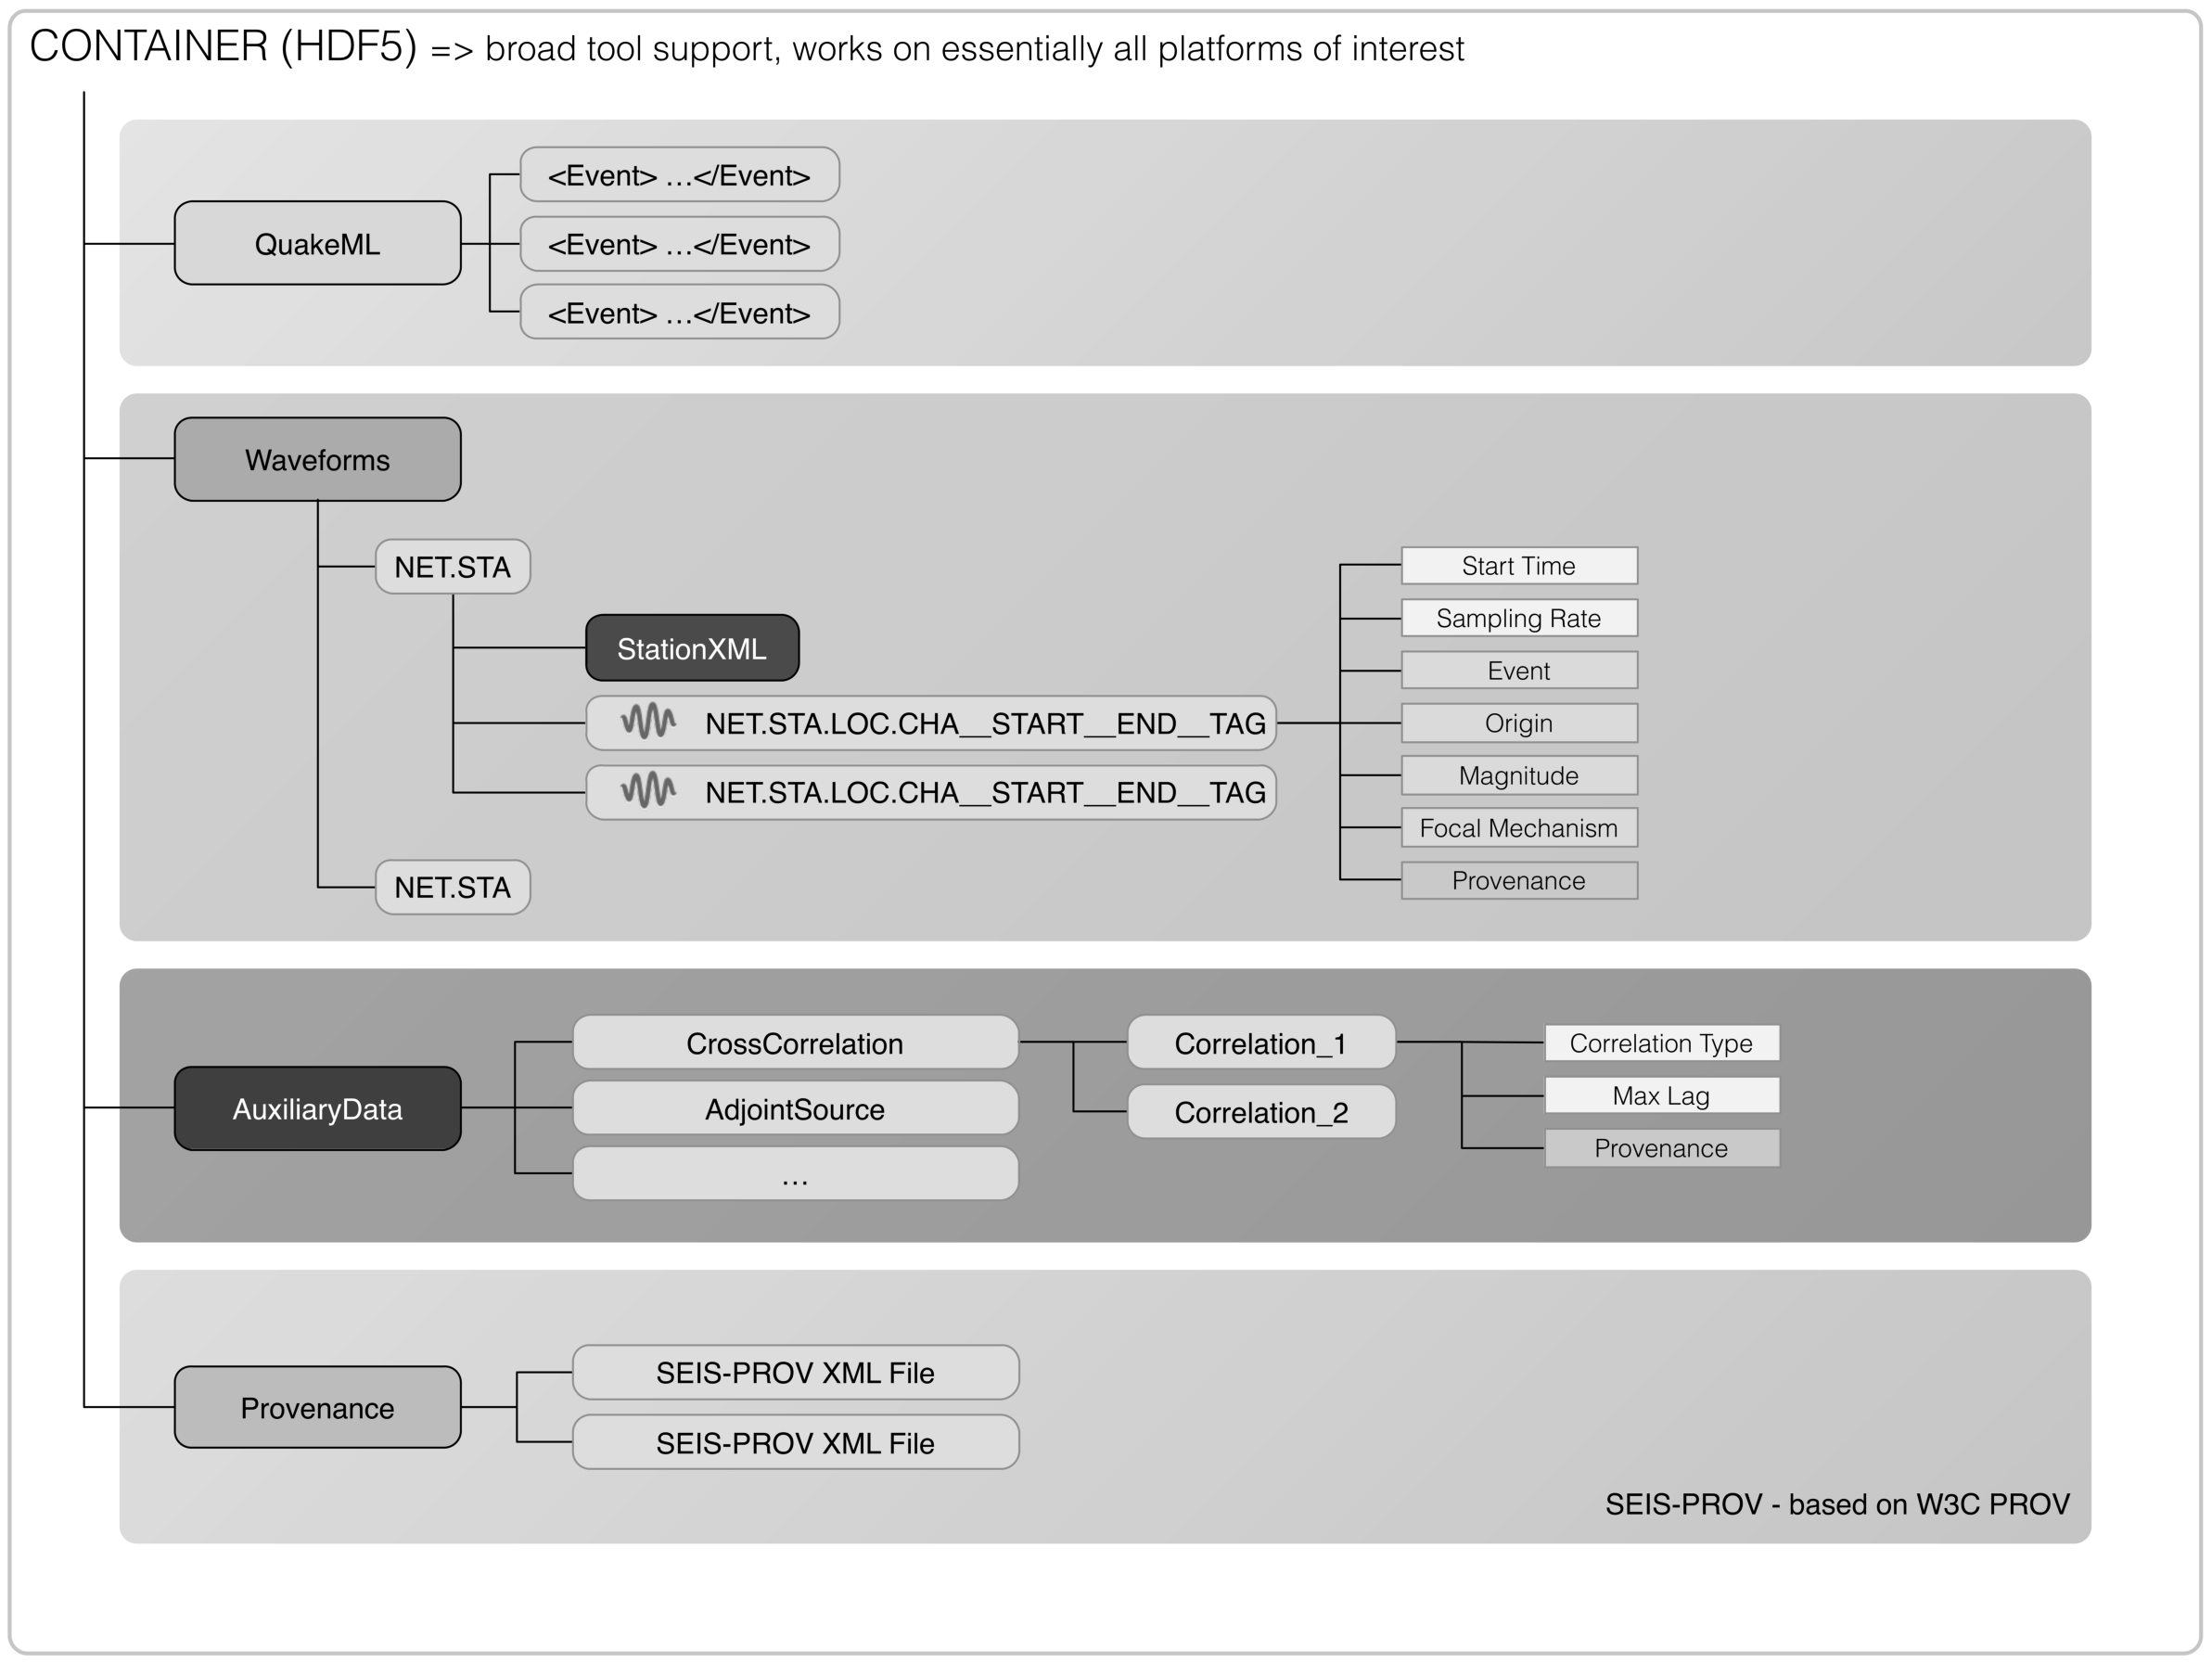
\includegraphics[width=0.8\textwidth]{ch-workflow/figures/ASDF_container_bw}
  \caption[Layout of the Adaptable Seismic Data Format]
  {Layout of the Adaptable Seismic Data Format, including earthquake
  event information, waveforms and station meta information, auxiliary data and
  provenance. In such layout, different types of data are grouped into
  one file and ready for later retrieval.}
  \label{fig:asdf_container}
\end{figure}

\subsection{Data Processing}

Global adjoint tomography is ideal for the ASDF data format.
First, the data volumes involved are massive, easily containing millions of
seismograms. Second, it necessitates sophisticated processing to turn raw data
into meaningful results. Here, we present a typical data processing workflow
occurring in full seismic waveform inversions with adjoint techniques
\cite{Tromp2005, Fichtner2006, Tape2010, zhu2012structure}.
The general idea also
translates to other types of tomography (see \cite{Liu2012} for a recent
review).

To enable a physically meaningful comparison between observed and synthetic
waveforms, time series need to be converted to the same units and filtered in a
way that ensures a comparable spectral content. This includes standard
processing steps like detrending, tapering, filtering, interpolating,
deconvolving the instrument response, and others. Subsequently, time windows in
which observed and simulated waveforms are sufficiently similar are selected and adjoint sources
are constructed from the data within these windows, see
Figure~\ref{fig:adjoint_workflow} for a graphical overview.

\begin{figure}[htb!]
  \centering
  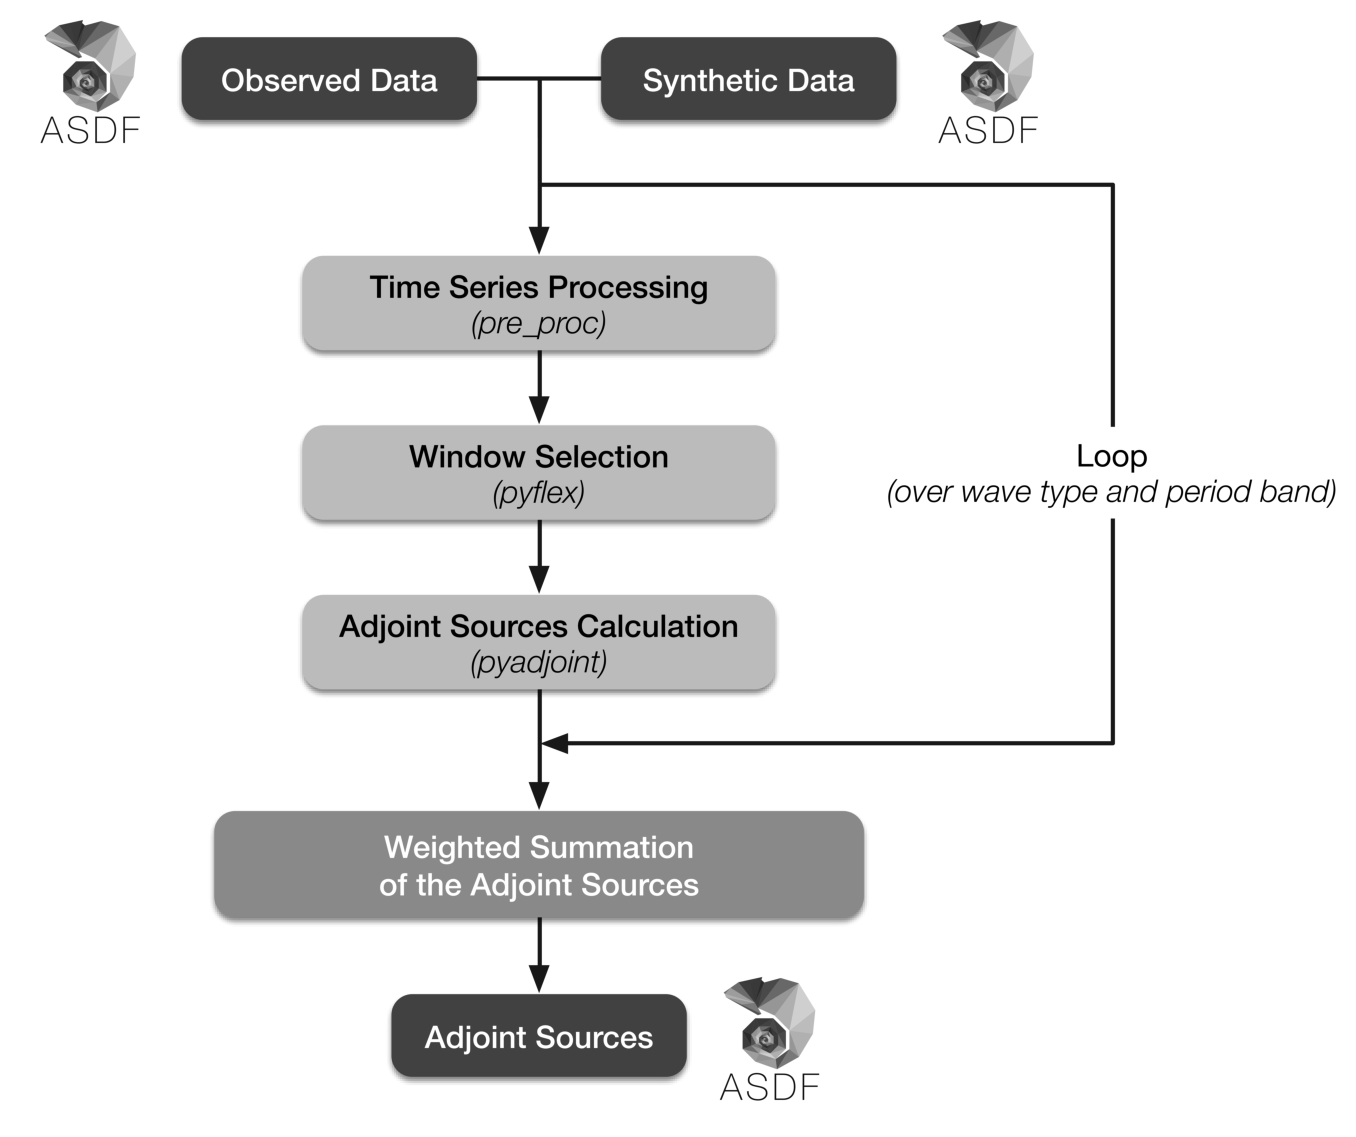
\includegraphics[width=0.8\textwidth]{ch-workflow/figures/adjoint_workflow_bw}
  \caption[Workflow of seismic data processing using ASDF]
  {Workflow of seismic data processing using ASDF. First, time
  series analysis is applied to raw observed and synthetic data to ensure a
  comparable spectral content at a later stage. Then, time windows are selected
  for pairs of processed observed and synthetic data, inside which
  measurement are made. Finally, adjoint sources are generated as the
  final pre-processing output. ASDF speeds up these tasks by using parallel processing (MPI).
  For each step, processing information is added to the provenance.}
  \label{fig:adjoint_workflow}
\end{figure}

The following is an account of our experiences and compares a legacy workflow
to one utilizing the ASDF format, demonstrating the latter's clear advantages.
Existing processing tools oftentimes work on pairs of SAC files, observed and
synthetic seismic data for the same component and station, and loop over all
seismic records associated with any given earthquake.
Given the large number of seismic receivers and earthquakes, the frequent read
and write operations on a very large number of single files create severe I/O
bottlenecks on modern compute platforms.
The implementation centered around ASDF shows superior scalability for
applications on high-performance computers: observed and synthetic seismograms
of a single event are stored in only two ASDF files, resulting in a
significantly reduced I/O load.  What is more, it is beneficial to keep meta
information in the same file. For example, one does not need to reach out for
separate files that keep track of the stations' instrument information or files
containing earthquake information, which greatly reduces the complexity of
operations and the possibility of making mistakes. Last but not least,
provenance information is kept to increase reproducibility and for future
reference.

Other than the data format itself, the data processing workflow benefits from the extensive
APIs provided by ASDF. ASDF is supported in the \texttt{SPECFEM3D\_GLOBE}
package \cite{KoTr02a}. Synthetic ASDF files are
directly generated, meaning synthetic data can seamlessly be fed as an input
into the workflow. To maximize performance, we rewrote our existing processing
tools. A big drawback in the old versions was that codes were written in
different languages and unable to communicate with each other easily. For
example, the SAC package was used for
signal processing and the Fortran based FLEXWIN program \cite{maggi2009automated} for
window selection.
In the new version we treat tasks as individual components in a single cohesive
workflow. Relying on the seismic analysis package ObsPy \cite{obspy2010}, we
re-developed all workflow components in Python. Therefore, all components
integrate with each other and stream data from one unit to the next. I/O only
happens at the very beginning, when we read the seismogram into memory, and at
the very end, when we write out the adjoint sources. All in all these changes
empower us to increase the scale of our inversions ---in terms of frequency
content, number of earthquakes, and number of stations--- and fully exploit
modern computational platforms.
